\documentclass[12pt,english,openany]{scrbook}  
\usepackage{amsmath,pifont}
\usepackage{amssymb,amsxtra}       
 \usepackage{commath}               
\setlength\parindent{0pt}
\usepackage{color, soul}
\usepackage[makeroom]{cancel}
\usepackage{MnSymbol,wasysym}
\usepackage{natbib}
\usepackage{graphicx}                                     


          
\title{MDOODZ6.0}
\author{MDOODZ Developper Team}
\subtitle{Documentation}
\subject{/*-----------------------*/}
\begin{document}
\maketitle
\tableofcontents

%---------------------------------------------------------------------------------------------------------------%
\addchap{Installation}
\section{Prequisites}

So far MDOODZ has been successfully built on LINUX/UNIX and MAC OS systems. 
The code can be built with GCC compiler from GNU (http://gcc.gnu.org) or with ICC compiler from Intel MKL library (https://software.intel.com/en-us/intel-mkl).
 \\ \\
The code relies on two libraries: 
\begin{enumerate}
\item SuiteSparse provides efficient linear algebra and matrix manipulation routines. It is available at: http://www.suitesparse.com \\
\item HDF5 is the main format for output files and is readable into MATLAB. It is available at: http://www.hdfgroup.org
\end{enumerate}

\section{Installation on Mac OS using MacPorts}

All components that are required to build the code can be installed via the MacPorts platform on Mac OS by the following steps:

\begin{enumerate}
\item Download the MacPorts platform following the instructions on the webpage: https://www.macports.org/install.php
\item Install the required components by opening a terminal window and type
\begin{enumerate}
\item sudo port install git
\item sudo port install gccX		(f.e., gcc7 for version 7)
\item sudo port install suitesparse
\item sudo port install hdf5
\end{enumerate}
\item Make sure the installed gcc compiler is active
\begin{enumerate}
\item sudo port select --list gcc  		(list of all installed versions of gcc)
\item sudo port select --set gcc mp-gccX	(activate gcc compiler version X)	
\end{enumerate}
\end{enumerate}

For a successful build the user has to link libraries and set certain environmental variables in the bash script named: ``.profile''			(usually located at /Users/YOUR\_USERNAME/) \\


If this file doesn�t exist, one has to create it. The first line of .profile has to be:
\begin{verbatim} 
\#!/usr/bin/env bash 
\end{verbatim}

Further, one has to set: 
\begin{verbatim} 
export HDF5\_USE\_FILE\_LOCKING='FALSE' 
\end{verbatim}

For the HDF5 libraries, to include the C path via: 
\begin{verbatim} 
export C\_INCLUDE\_PATH=/opt/local/include 
\end{verbatim}

And finally link the libraries: 
\begin{verbatim} 
export LIBRARY\_PATH=/opt/local/lib
\end{verbatim}

Note that .profile is executed once each time a new terminal session is started, thus it is very useful to set frequently used commands, global variables etc. in this file to avoid finger pain.

The user has installed all required components and linked all libraries correctly now. 
Prior to compilation, one needs to figure out which makefile to use (or to design your own makefile). Examples of makefiles valid for different systems are available in the Makefiles folder.

The user needs to copy the appropriate makefile into the source folder (../) and to rename it ``makefile\_XXXX'' into simply "makefile". One has to be careful and set the compiler accordingly in the makefile like:
\begin{verbatim} 
		# Compiler
		ifeq ($(GNU),yes)
        		CC=/opt/local/bin/gcc-mp-7
		#endif
\end{verbatim}

\section{Source files}

The source consists of one ``.h'' file and a several ``.c'' files.
The file ``head.h''' contains the definition of data structures uses in the codes as well as function headers.
The ``.c'' files contains all the functions of the codes. Key files are for example ``Main\_MDOODZ\_GREAT.c'' that contains the main function, ``flow\_laws.c'' that contains the flow law database, and the file ``set\_XXXX.c'' in which user-defined setups are constructed (XXXX is a user defined name). 
For compiling the source a ``makefile'' is provided.
In order to run a simulation, an additional "XXXX.txt" that contains run-time parameters (solver options, material properties, key parameters) is also required. 


\section{Compilation}

\textbf{Compilation flags}: 
\begin{itemize}
\item MODEL\_PATH corresponds to the path towards the directory containing the ``set\_XXXX.c''. 
\item MODEL corresponds to the model name, as for ``set\_XXXX.c'' and the "XXXX.txt" files.
\item OPT: optimized built should be set to yes or no.
\item OMP: OpenMP Parallelization should be set to yes or no.
\end{itemize}

\textbf{Non-optimized build:}  
\begin{verbatim} 
make clean all MODEL_PATH=BENCHMARKS MODEL=SubBenchCase1 OPT=no OMP=no
\end{verbatim}
\textbf{Optimized build:}  
\begin{verbatim} 
make clean all MODEL_PATH=BENCHMARKS MODEL=SubBenchCase1 OPT=yes OMP=yes
\end{verbatim}
%---------------------------------------------------------------------------------------------------------------%
\addchap{Benchmarks}
\section{Subduction benchmark case 1, \citet{Schmeling08}}

\begin{figure}[ht!]
\centerline{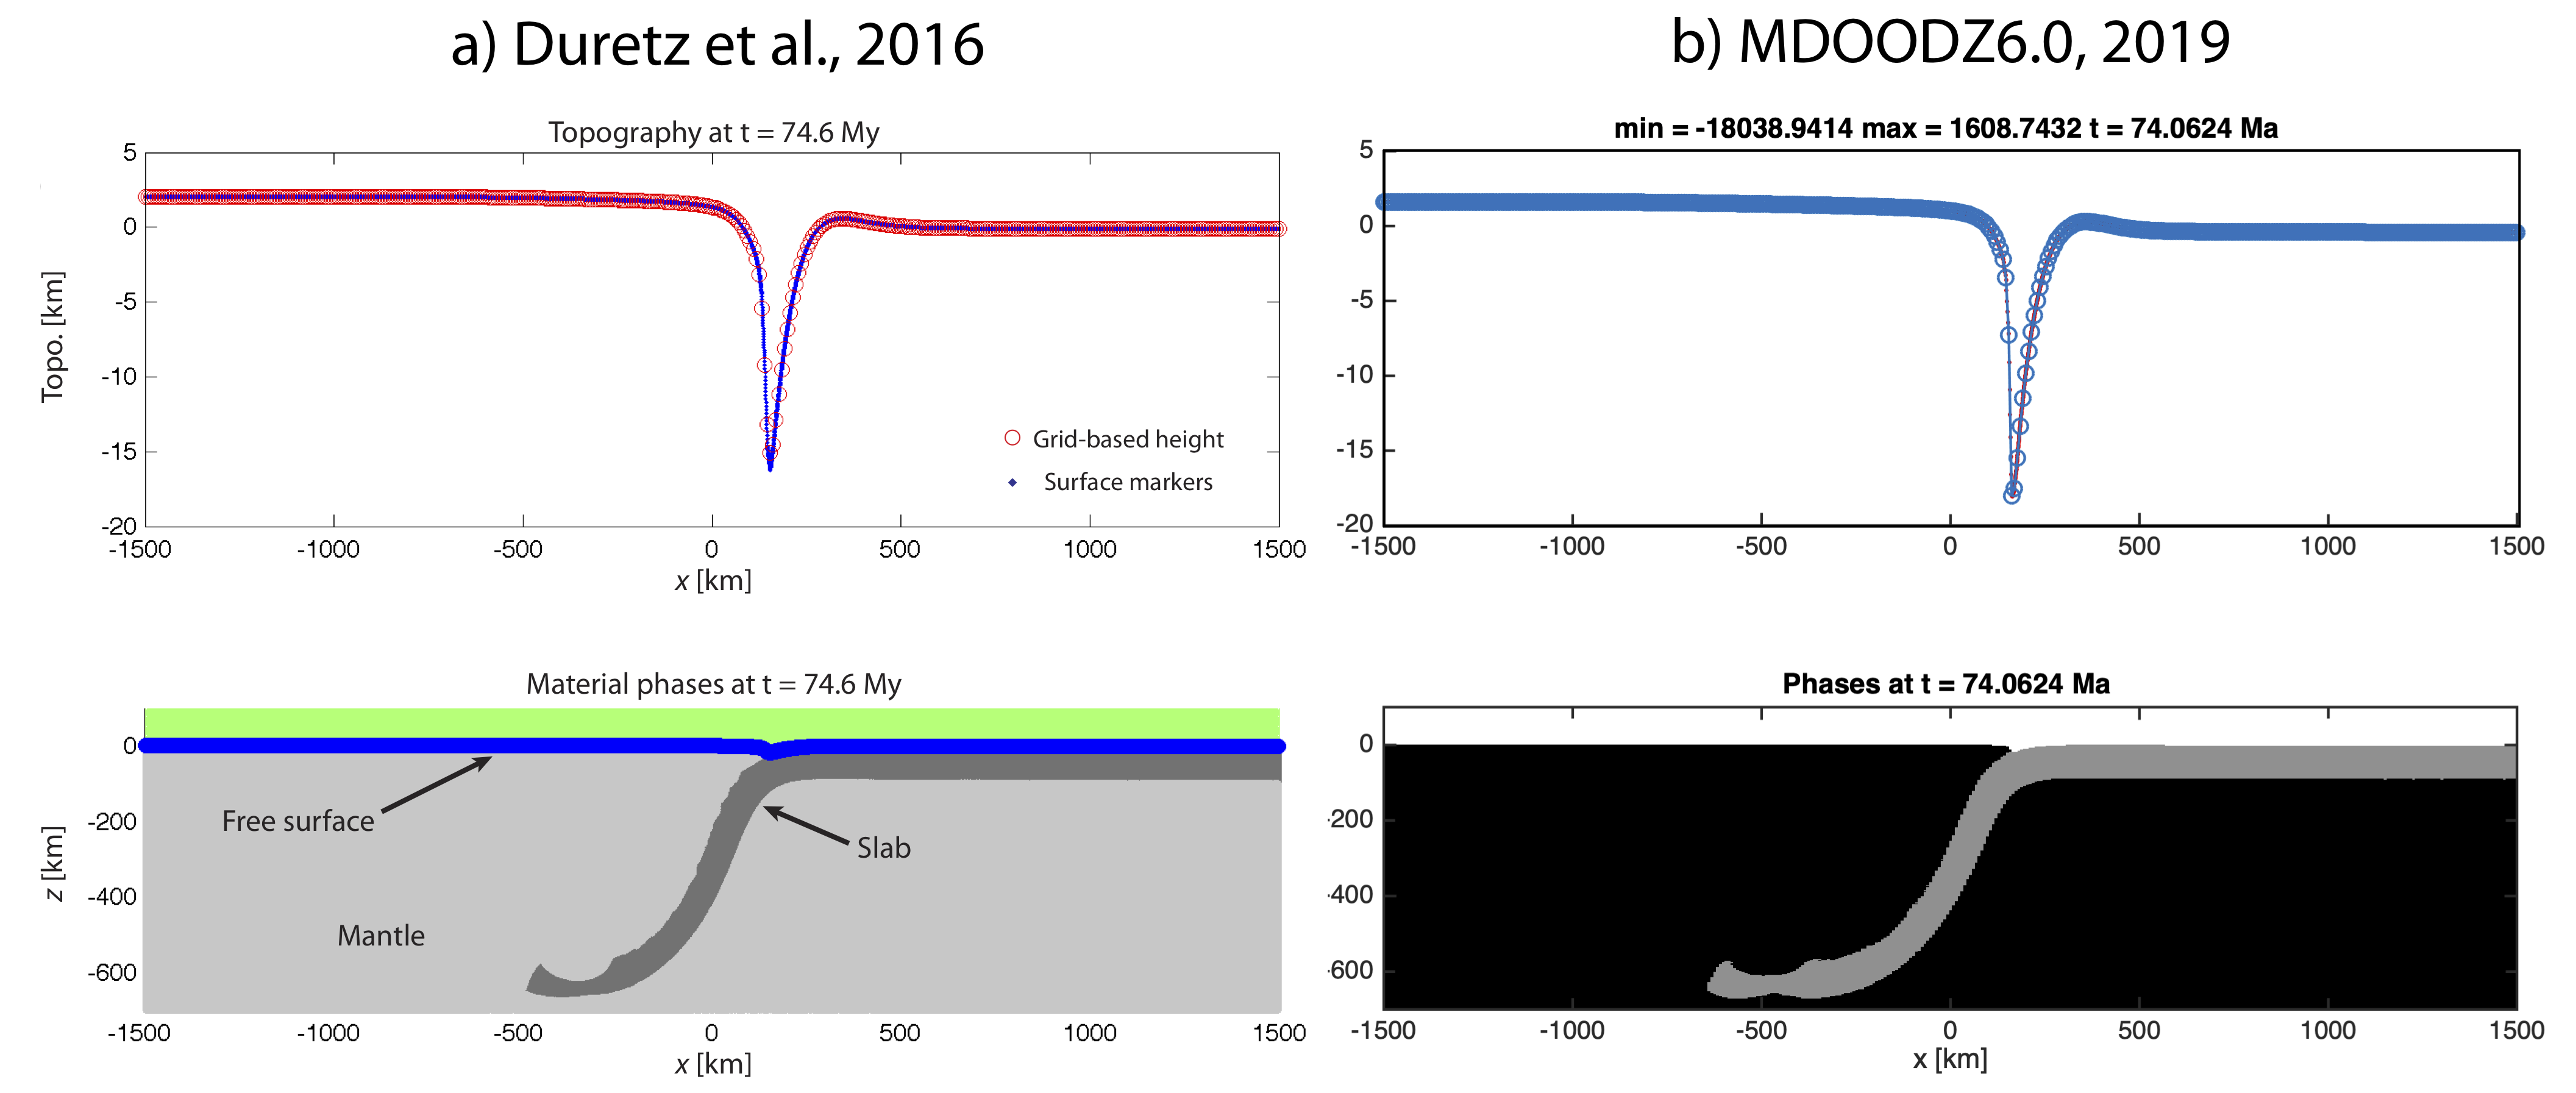
\includegraphics[height=3.0in]{./Figures/SubBench1_MDOODZ}}
\caption{Comparison between results of \citet{Duretz16} and current version of MDOODZ. After $\sim76$ My, The minimum bathymetry is $\sim-16$ km and trench position is $\sim150$ km.}
\label{SubBench1}
\end{figure}

\section{Subduction benchmark case 3, \citet{Schmeling08}}

\begin{figure}[ht!]
\centerline{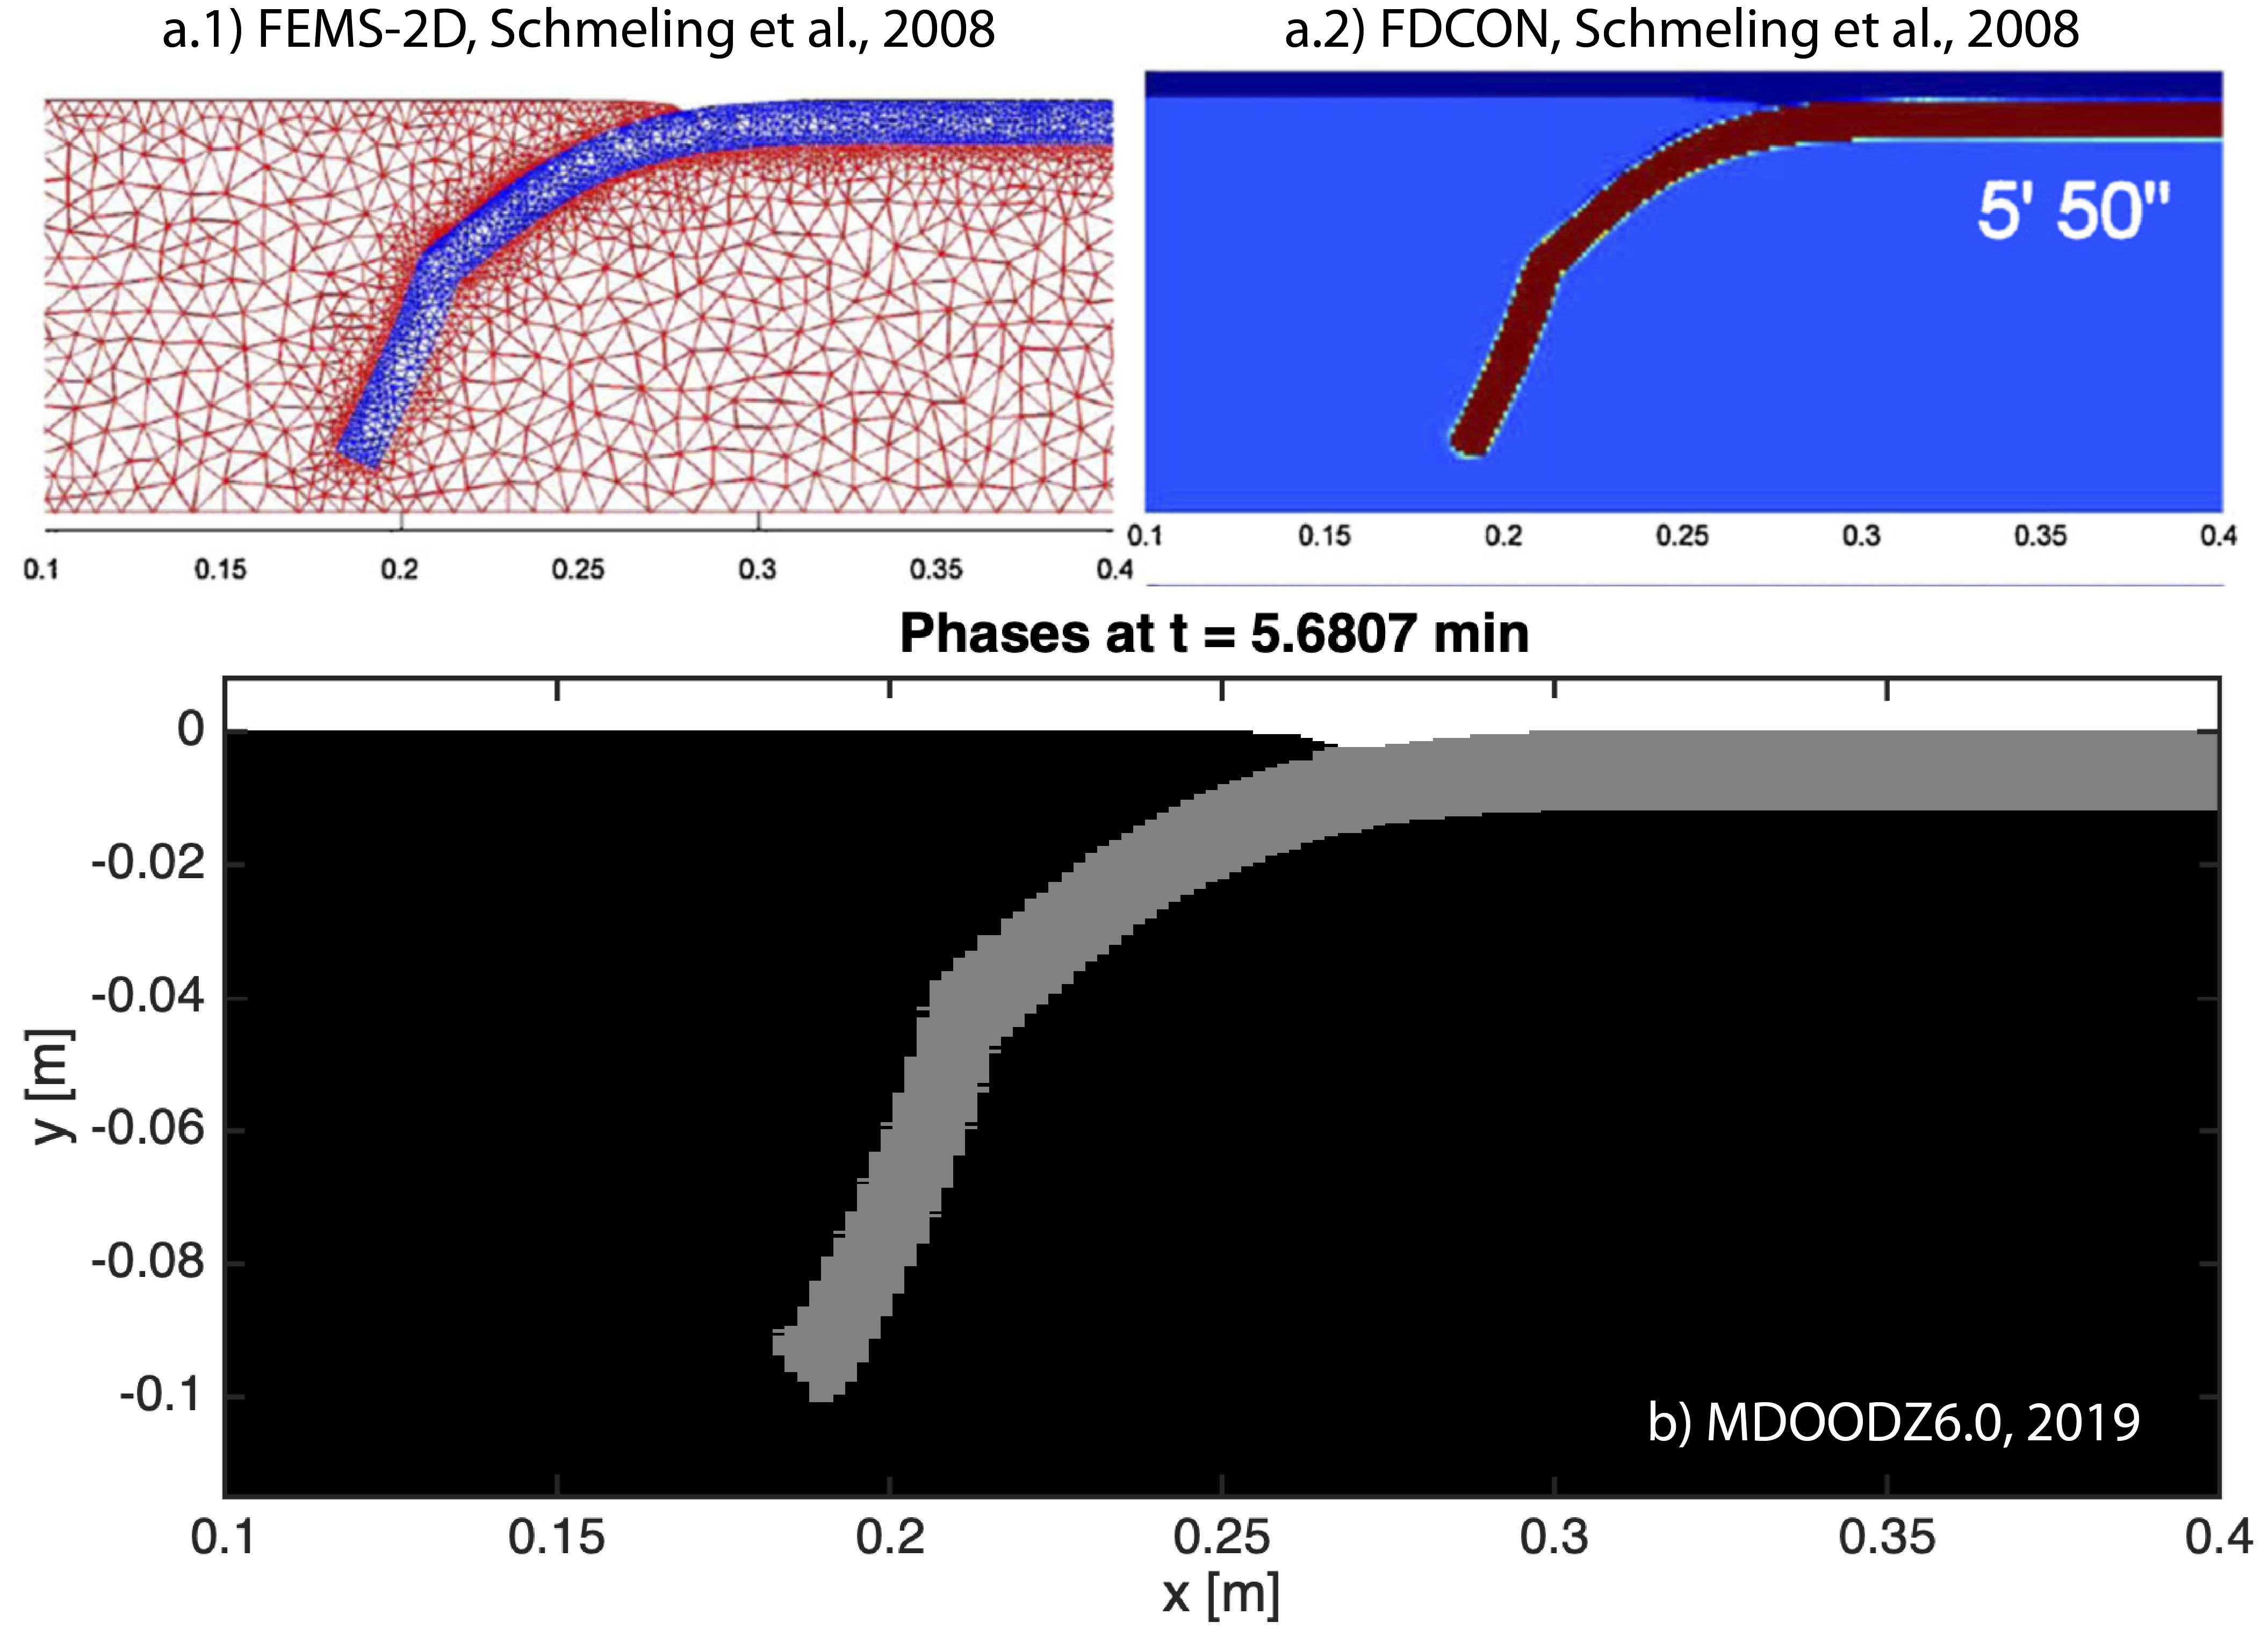
\includegraphics[height=3.0in]{./Figures/SubBench3_MDOODZ}}
\caption{Comparison between results of \citet{Schmeling08} and current version of MDOODZ. After $\sim5.7$ min.}
\label{SubBench3}
\end{figure}

%---------------------------------------------------------------------------------------------------------------%
\addchap{Matlab Examples}
\section{Finite Strain ellipsoid and tensor and vector rotation}


\begin{figure}[ht!]
\centerline{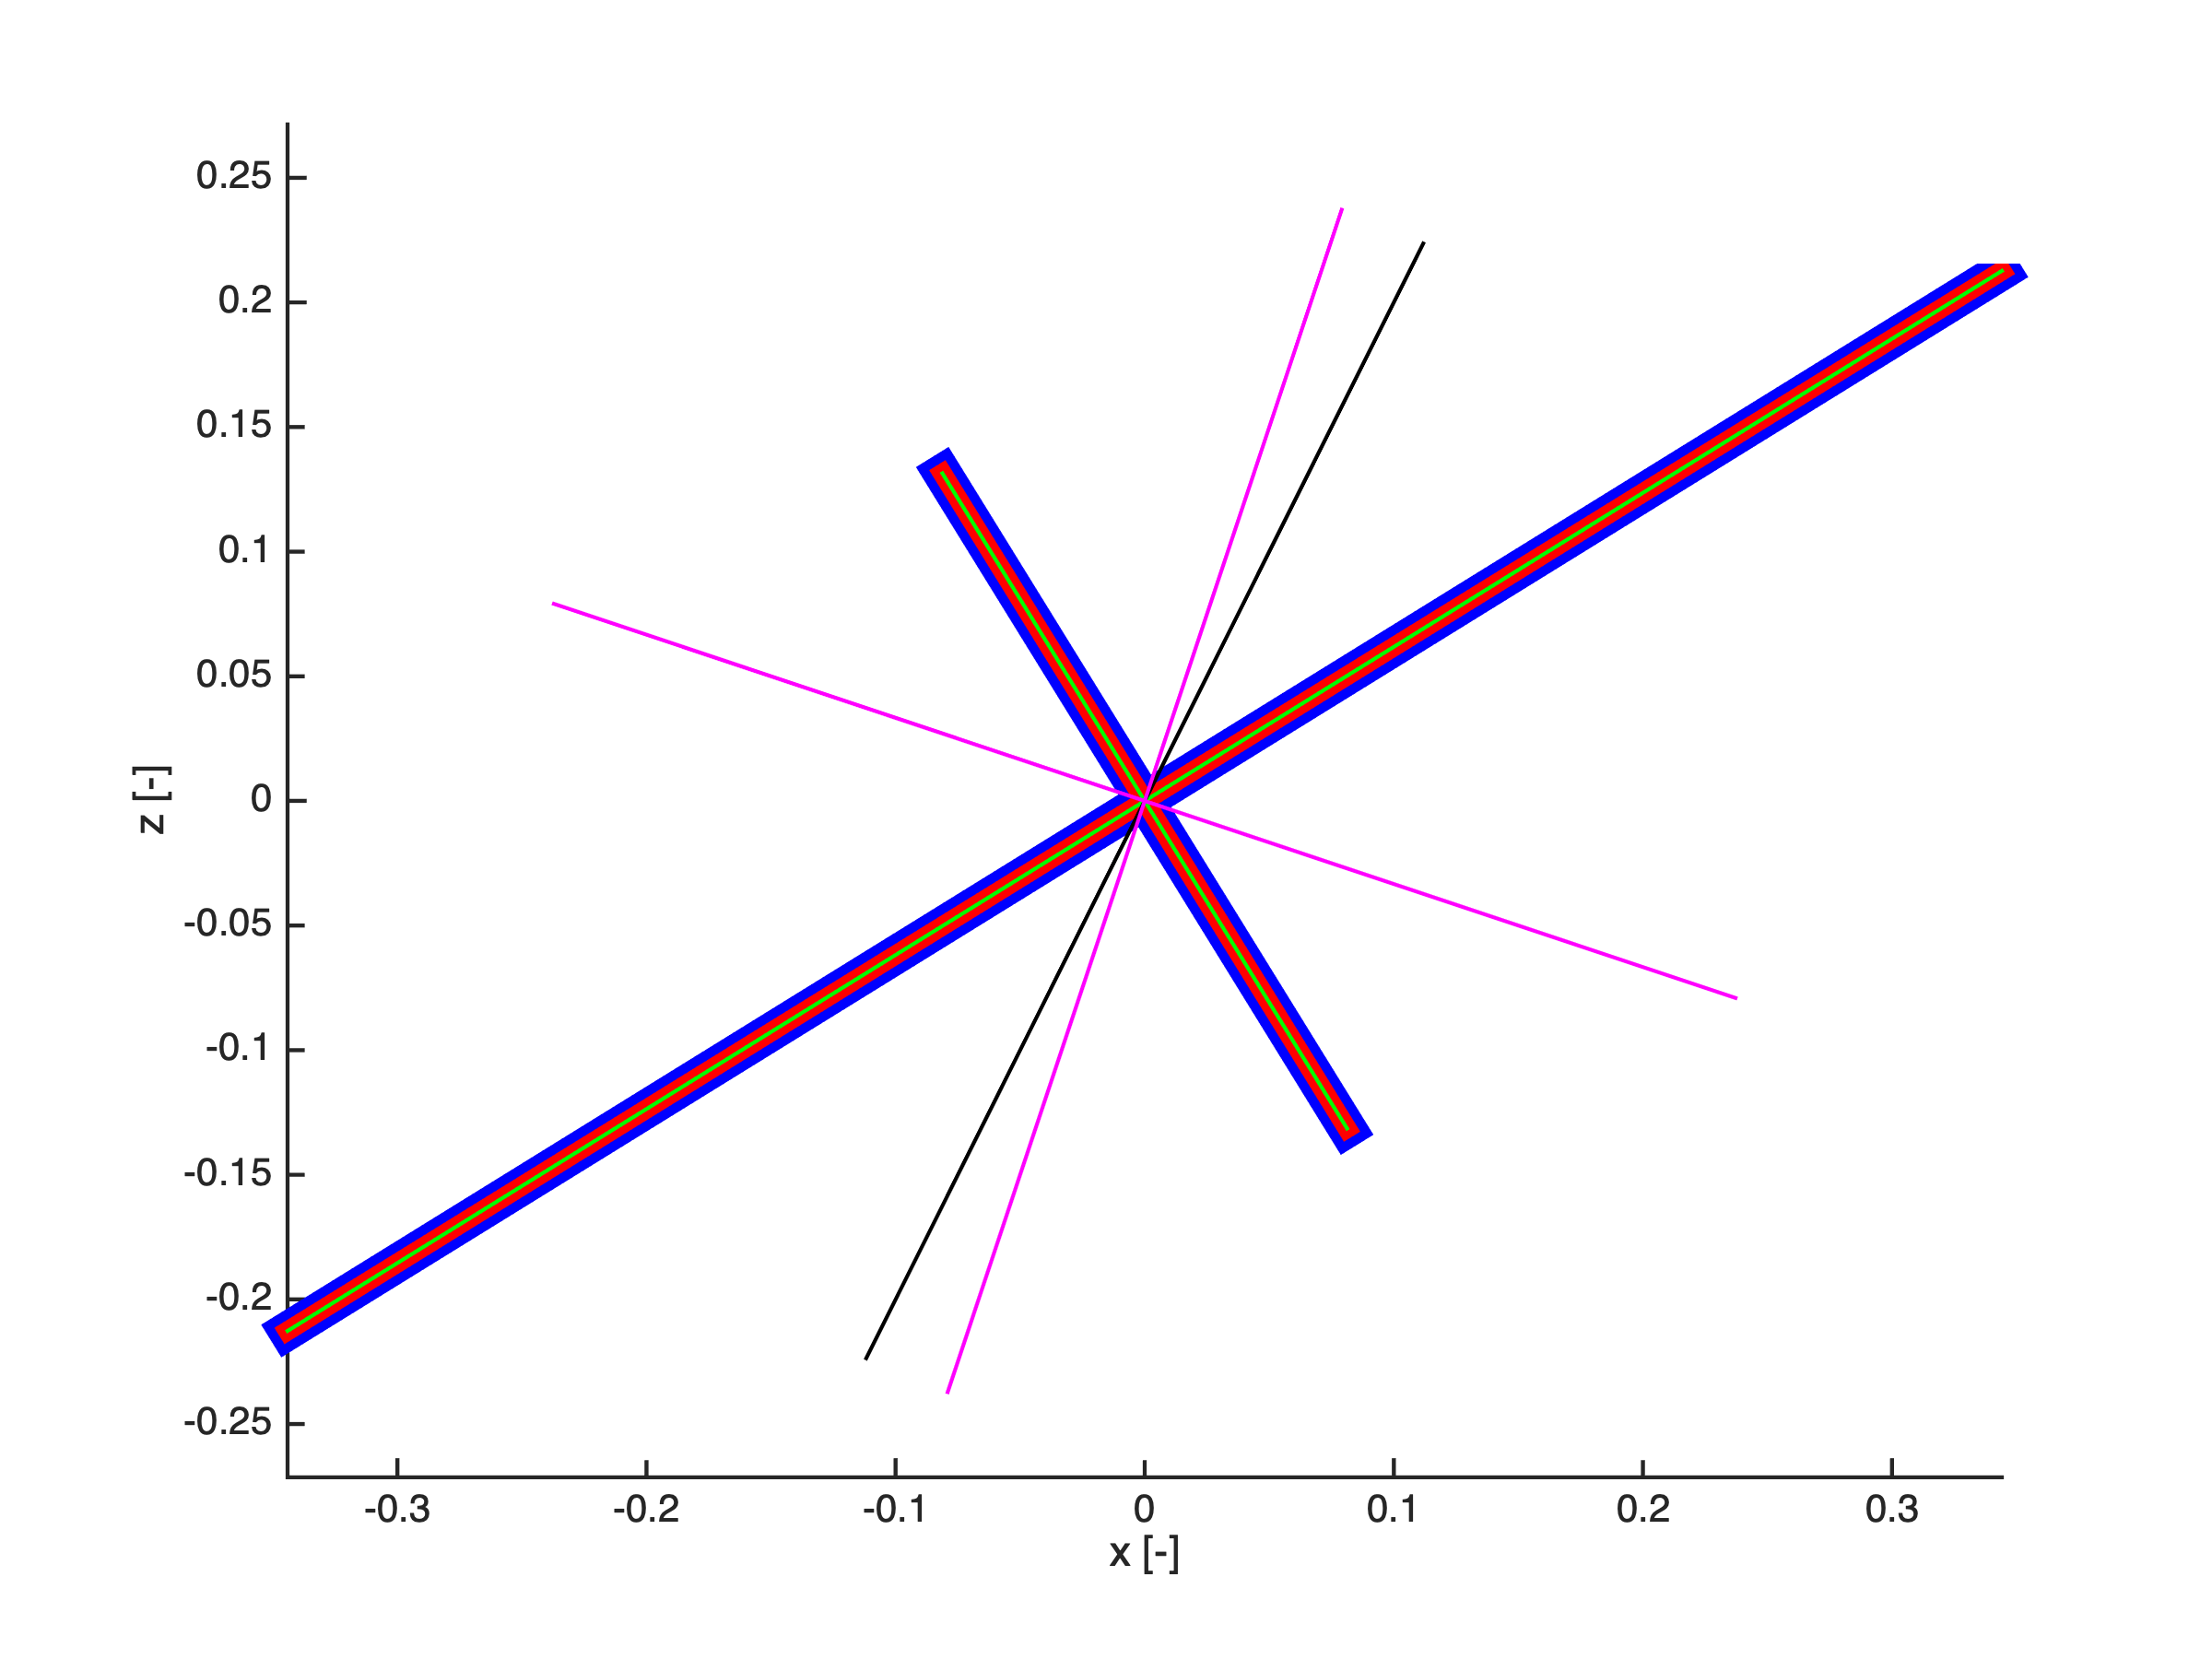
\includegraphics[height=4.0in]{./Figures/FiniteStrainRotation}}
\caption{Simple shear deformation with $\gamma = 1.0$. Finite strain principal axis (thick lines). Rotated tensor principal axis (pink lines) originally oriented at 45 degrees. Rotated vector (black line) originally vertical.}
\label{FiniteStrainRotation}
\end{figure}

%---------------------------------------------------------------------------------------------------------------%
\addchap{Python Code Generation}
\bibliographystyle{plainnat}
\bibliography{references} 
\end{document}

